\documentclass[12pt]{report}
\usepackage[utf8x]{inputenc}
\usepackage[russian]{babel}
\usepackage{listings}
\usepackage{graphicx}
\usepackage{amsmath,amsfonts,amssymb,amsthm,mathtools} 
\usepackage{pgfplots}
\usepackage{filecontents}
\usepackage{indentfirst}
\usepackage{eucal}
\usepackage{float}
\usepackage{caption}
\usepackage{enumitem}
\usepackage{multirow}
\frenchspacing


% Для листинга кода:
\lstset{ %
language=c,        
extendedchars=\true,     % выбор языка для подсветки (здесь это С)
basicstyle=\small\sffamily, % размер и начертание шрифта для подсветки кода
numbers=left,               % где поставить нумерацию строк (слева\справа)
numberstyle=\tiny,           % размер шрифта для номеров строк
stepnumber=1,                   % размер шага между двумя номерами строк
numbersep=5pt,                % как далеко отстоят номера строк от подсвечиваемого кода
showspaces=false,            % показывать или нет пробелы специальными отступами
showstringspaces=false,      % показывать или нет пробелы в строках
showtabs=false,             % показывать или нет табуляцию в строках
frame=single,              % рисовать рамку вокруг кода
tabsize=2,                 % размер табуляции по умолчанию равен 2 пробелам
captionpos=t,              % позиция заголовка вверху [t] или внизу [b] 
breaklines=true,           % автоматически переносить строки (да\нет)
breakatwhitespace=false, % переносить строки только если есть пробел
escapeinside={\#*}{*)},   % если нужно добавить комментарии в коде
}


\usepackage[left=3cm,right=1cm, top=2cm,bottom=2cm,bindingoffset=0cm]{geometry}
% Для измененных титулов глав:
\usepackage{titlesec, blindtext, color} % подключаем нужные пакеты
\definecolor{gray75}{gray}{0.75} % определяем цвет
\newcommand{\hsp}{\hspace{20pt}} % длина линии в 20pt
% titleformat определяет стиль
\usepackage{titlesec}

\lstdefinestyle{mystyle}{
    language=Lisp,
	backgroundcolor=\color{white},
	basicstyle=\footnotesize\ttfamily,
	keywordstyle=\color{blue},
	stringstyle=\color{red},
	commentstyle=\color{gray},
	directivestyle=\color{orange},
	numbers=left,
	numberstyle=\tiny,
	stepnumber=1,
	numbersep=5pt,
	frame=single,
	tabsize=4,
	captionpos=t,
	breaklines=true,
	breakatwhitespace=true,
	escapeinside={\#*}{*)},
	morecomment=[l][\color{magenta}]{\#},
	columns=fullflexible
}

\lstset{style=mystyle}

\titleformat{\section}[block]
{\Large\filcenter\newpage\MakeUppercase}
  {\thesection}
  {1em}
  {\MakeUppercase}{}

\linespread{1.25}
\setlength\parindent{5ex}

\begin{document}
\thispagestyle{empty}
\begin{titlepage}
	\noindent \begin{minipage}{0.15\textwidth}
	
\includegraphics[width=\linewidth]{./inc/img/b_logo.jpg}
	\end{minipage}
	\noindent\begin{minipage}{0.9\textwidth}\centering
		\textbf{Министерство науки и высшего образования Российской Федерации}\\
		\textbf{Федеральное государственное бюджетное образовательное учреждение высшего образования}\\
		\textbf{«Московский государственный технический университет имени Н.Э.~Баумана}\\
		\textbf{(национальный исследовательский университет)»}\\
		\textbf{(МГТУ им. Н.Э. Баумана)}
	\end{minipage}
	
	\noindent\rule{18cm}{3pt}
	\newline\newline
	\noindent ФАКУЛЬТЕТ $\underline{\text{«Информатика и системы управления»}}$ \newline\newline
	\noindent КАФЕДРА $\underline{\text{«Программное обеспечение ЭВМ и информационные технологии»}}$\newline\newline\newline\newline\newline
	
  \begin{center}
        \Large\textbf{Отчет по лабораторной работе №1 по курсу "Математическая статистика"}
    \end{center}
	
	\noindent\textbf{Тема} $\underline{\text{Гистограмма и эмпирическая функция распределения}}$\newline\newline
	\noindent\textbf{Студент} $\underline{\text{Варин Д.В.}}$\newline\newline
	\noindent\textbf{Группа} $\underline{\text{ИУ7-66Б}}$\newline\newline
	\noindent\textbf{Оценка (баллы)} $\underline{\text{~~~~~~~~~~~~~~~~~~~~~~~~~~~}}$\newline\newline
	\noindent\textbf{Преподаватели} $\underline{\text{Андреева Т.В.}}$\newline\newline\newline
	
	\begin{center}
		\vfill
		Москва~---~\the\year
		~г.
	\end{center}
\end{titlepage}

\renewcommand{\thefigure}{\thesection.\arabic{figure}} 
\renewcommand{\thetable}{\thesection.\arabic{table}} 
\renewcommand{\thelstlisting}{\thesection.\arabic{lstlisting}} 


\renewcommand*\thesection{\arabic{section}}


\section{Задание}

\textbf{Цель работы:} построение гистограммы и эмпирической функции распределения.

\begin{enumerate}
    \item Для выборки объёма $n$ из генеральной совокупности $X$ реализовать в виде программы на ЭВМ
        \begin{enumerate}
            \item вычисление максимального значения $M_{\max}$ и минимального значения $M_{\min}$;
            \item размаха $R$ выборки;
            \item вычисление оценок $\hat\mu$ и $S^2$ математического ожидания $MX$ и дисперсии $DX$;
            \item группировку значений выборки в $m = [\log_2 n] + 2$ интервала;
            \item построение на одной координатной плоскости гистограммы и графика функции плотности распределения вероятностей нормальной случайной величины с математическим ожиданием $\hat{\mu}$ и дисперсией $S^2$;
            \item построение на другой координатной плоскости графика эмпирической функции распределения и функции распределения нормальной случайной величины с математическим ожиданием $\hat{\mu}$ и дисперсией $S^2$.
        \end{enumerate}
    \item Провести вычисления и построить графики для выборки из индивидуального варианта.
\end{enumerate}

\section{Теоретические сведения}

\subsection{Формулы для вычисления величин}

\subsubsection{Минимальное и максимальное значения выборки}
\begin{equation}
    \begin{aligned}
        M_{\max} = X_{(n)}\\
        M_{\min} = X_{(1)}
    \end{aligned}
\end{equation}

\subsubsection{Размах выборки}
\begin{equation}
    R = M_{\max} - M_{\min}.
\end{equation}

\subsubsection{Оценки математического ожидания и исправленной дисперсии}
\begin{equation}
    \begin{aligned}
    \hat\mu(\vec X_n) &= \frac 1n \sum_{i=1}^n X_i\\
    S^2(\vec X_n) &= \frac 1{n-1} \sum_{i=1}^n (X_i-\overline X_n)^2
    \end{aligned}
\end{equation}

\section{Определение эмпирической плотности и гистограммы}

Пусть $\vec x$ -- выборка из генеральной совокупности $X$. Если объем $n$ этой выборки велик, то значения $x_i$ группируют в интервальный статистический ряд. Для этого отрезок $J = [x_{(1)}, x_{(n)}]$ делят на $m$ равновеликих частей:

\begin{equation*}
    J_i = [x_{(1)} + (i - 1) \cdot \Delta, x_{(1)} + i \cdot \Delta), i = \overline{1; m - 1},
\end{equation*}

\begin{equation*}
    J_{m} = [x_{(1)} + (m - 1) \cdot \Delta, x_{(n)}],
\end{equation*}

\begin{equation*}
    \Delta = \frac{|J|}{m} = \displaystyle\frac{x_{(n)} - x_{(1)}}{m}.
\end{equation*}

Интервальным статистическим рядом называют таблицу:

\begin{table}[htb]
    \centering
    \begin{tabular}{|c|c|c|c|c|}
        \hline
        $J_1$ & ... & $J_i$ & ... & $J_m$ \\
        \hline
        $n_1$ & ... & $n_i$ & ... & $n_m$ \\
        \hline
    \end{tabular}
\end{table}

где $n_i$ -- количество элементов выборки $\vec x$, которые $\in J_i$.

Обычно выборку разбивают на $m=[\log_2n]+2$ интервалов, где $n$ -- размер выборки.

Гистограмма -- это график эмпирической плотности. 

\textit{Эмпирической плотностью}, отвечающей выборке $\vec x$, называют функцию:
\begin{equation}
    \hat f(x) =
    \begin{cases}
        \displaystyle\frac{n_i}{n \Delta}, \quad x \in J_i, i = \overline{1; m}, \\
        0, \quad \text{ иначе,} \\
    \end{cases}
\end{equation}
где $J_i$ -- полуинтервал статистического ряда, $n_i$ -- количество элементов выборки, входящих в полуинтервал, $n$ -- количество элементов выборки.


\section{Определение эмпирической функции распределения}

Пусть $\vec x = (x_1, ..., x_n)$ -- выборка из генеральной совокупности $X$. Обозначим $n(x, \vec x)$ -- число элементов вектора $\vec x$, которые имеют значения меньше $x$.

\textit{Эмпирической функцией распределения} называют функцию $F_n: \mathbb{R} \to \mathbb{R}$, определенную как: 

\begin{equation}
    F_n(x) = \frac{n(x, \vec x)}{n}.
\end{equation}

Замечание. 
\begin{enumerate}
    \item  Обладает всеми свойствами функции распределения; 
    \item  Кусочно-постоянна;
    \item Ксли все элементы вектора различны, то
    
    \begin{equation}
    F(x) =
    \begin{cases}
    0, \quad x \leq x_{(1)}, \\
        \displaystyle\frac{i}{n}, \quad x_{(i)} < x \leq  x_{(i+1)},\\
        1, \quad  x > x_{(n)}. \\
    \end{cases}.
\end{equation}
\end{enumerate}

\section{Результат работы}

Вариант 3

\subsection{Код программы}

\begin{lstlisting}
function main()
    pkg load statistics

    function myhist()

        centers = zeros(1, m);
        heights = zeros(1, m);

        for i = 1:m
            heights(i) = counts(i) / (n * delta);
        endfor

        for i = 1:m
            centers(i) = bins(i + 1) - (delta / 2);
        endfor

        fprintf("Высоты столбцов гистограммы:\n");
        for i = 1:m
            fprintf("%d-ый столбец : %f\n", i, heights(i));
        endfor

        set(gca, "xtick", bins);
        set(gca, "ytick", heights);
        set(gca, "xlim", [min(bins) - 1, max(bins) + 1]);
        bar(centers, heights, 1);
        
        nodes = (m_min - 3):(S / 250):(m_max + 3);
        %nodes = 0:(S / 250):(m_max + 5);
        X_pdf = normpdf(nodes, mu, sqrt(S));
        plot(nodes, X_pdf, "r");
    end

    function mycdf()

        heights = zeros(1, m + 2);
        bins = [(min(bins) - 0.5) bins];
        counts = [0 counts 0];

        acc = 0;
        m = m + 2
        for i = 2:m
            acc = acc + counts(i);
            heights(i) = acc / n;
        end

        nodes = (m_min):(S / 250):(m_max);
        X_cdf = normcdf(nodes, mu, sqrt(S));
        plot(nodes, X_cdf, "r");

        for i = 2:m
            fprintf("x = %f : F(x) = %f\n", bins(i), heights(i));
        end

        set(gca, "xtick", bins);
        set(gca, "ylim", [0, 1.1]);
        set(gca, "ytick", heights);
        stairs(bins, heights);
    end
    
    X = [-0.45,-0.33,2.92,-1.25,-1.20,0.05,-0.53,-0.19,1.49,0.67,0.22,1.23,0.50,-0.92,...
          0.90,-1.52,-0.15,-1.24,-0.47,-0.45,0.18,-0.05,1.58,1.74,2.37,-0.24,-1.34,1.05,...
          1.28,1.37,1.18,0.22,0.11,0.28,-0.64,-0.39,-1.77,-1.61,0.47,0.77,-0.27,-1.19,-0.25,...
          1.04,-0.16,0.42,0.29,0.10,1.04,0.43,-0.67,0.41,-0.62,-1.49,1.46,-2.77,2.09,0.88,...
          -0.36,-0.71,-0.62,1.34,-0.78,-0.15,2.69,0.92,1.68,-0.12,0.34,0.74,1.72,1.24,0.23,...
          0.76,0.87,-1.52,0.63,-0.56,0.83,0.31,-0.18,0.99,-1.01,0.58,1.21,-1.51,0.65,0.35,...
          -0.37,-0.50,-0.73,0.63,0.33,1.56,-0.98,0.85,0.56,-1.07,1.47,1.44,1.91,0.24,1.34,...
          0.99,1.27,0.11,0.22,-0.25,0.35,-0.03,-0.56,-0.79,2.41,-0.45,-0.44,0.07,0.64,0.69,...
          0.10,-0.28]
   
    X = sort(X);

    
    m_max = max(X);
    m_min = min(X);
    fprintf("----------------------------------------\n");
    fprintf("1. Максимальное значение выборки: M_max = %f.\n", m_max);
    fprintf("   Минимальное значение выборки:  M_min = %f.\n", m_min);
    fprintf("----------------------------------------\n");

    
    r = m_max - m_min;
    fprintf("2. Размах выборки: R = %f.\n", r);
    fprintf("----------------------------------------\n");

    
    n = length(X);
    mu = sum(X) / n;
    S = sum((X - mu).^2) / (n - 1);
    fprintf("3. Оценка математического ожидания: m = %f.\n", mu);
    fprintf("   Оценка дисперсии: S^2 = %f.\n", S);
    fprintf("----------------------------------------\n");

    
    m = floor(log2(n)) + 2;
    bins = [];
    cur = m_min;
    delta = r / m 

    for i = 1:(m + 1)
        bins(i) = cur;
        cur = cur + delta;
    end

    eps = 1e-6;
    counts = [];

    for i = 1:(m - 1)
        cur = 0;

        for j = 1:n
            if ((X(j) - eps) > bins(i) || abs(bins(i) - X(j)) < eps) && X(j) < (bins(i + 1) - eps)
                cur = cur + 1;
            endif
        endfor

        counts(i) = cur;
    endfor

    cur = 0;
    for i = 1:n
        if (bins(m) < X(i) || abs(bins(m) - X(i)) < eps) && (X(i) < bins(m + 1) || abs(bins(m + 1) - X(i)) < eps)
            cur = cur + 1;
        endif
    endfor

    counts(m) = cur;

    fprintf("4. Группировка значений выборки в %d интервалов:\n", m);
    for i = 1:(m)
        fprintf("Интервал №%d [%f : %f) - %d значений из выборки.\n", i, bins(i), bins(i + 1), counts(i));
    end
    fprintf("----------------------------------------\n");


    fprintf("5. Построение гистограммы и графика функции плотности распределения нормальной СВ.\n");
    figure;
    hold on;
    grid on;
    myhist();
    xlabel('X')
    ylabel('P')
    print -djpg hist.jpg
    hold off;
    fprintf("----------------------------------------\n");

    fprintf("6. Построение графика эмпирической функции распределения и функции распределения нормальной СВ.\n");
    figure;
    hold on;
    grid on;
    mycdf(X, bins, counts);
    xlabel('X')
    ylabel('F')
    print -djpg cdf.jpg
    hold off;
end

main()
\end{lstlisting}

\section{Результаты расчётов}

\begin{equation*}
M_{\min} = -2.77 \\
\end{equation*}
\begin{equation*}
M_{\max} = 2.92 \\
\end{equation*}
\begin{equation*}
    R = 5.69 \\
\end{equation*}
\begin{equation*}
    \hat\mu(\vec x_n) = 0.23225 \\
\end{equation*}
\begin{equation*}
    S^2(\vec x_n) = 1.0406 \\
\end{equation*}
\begin{equation*}
    m = 8
\end{equation*}

[-2.77; -2.06) -        1


[-2.06; -1.35) -        6

[-1.35; -0.64) -       15

[-0.64;  0.07) -       30

[ 0.07;  0.79) -       33

[ 0.79;  1.50) -       24

[ 1.50;  2.21) -        7


[ 2.21,  2.92] -        4

\newpage
\begin{figure}[H]
	\begin{center}
		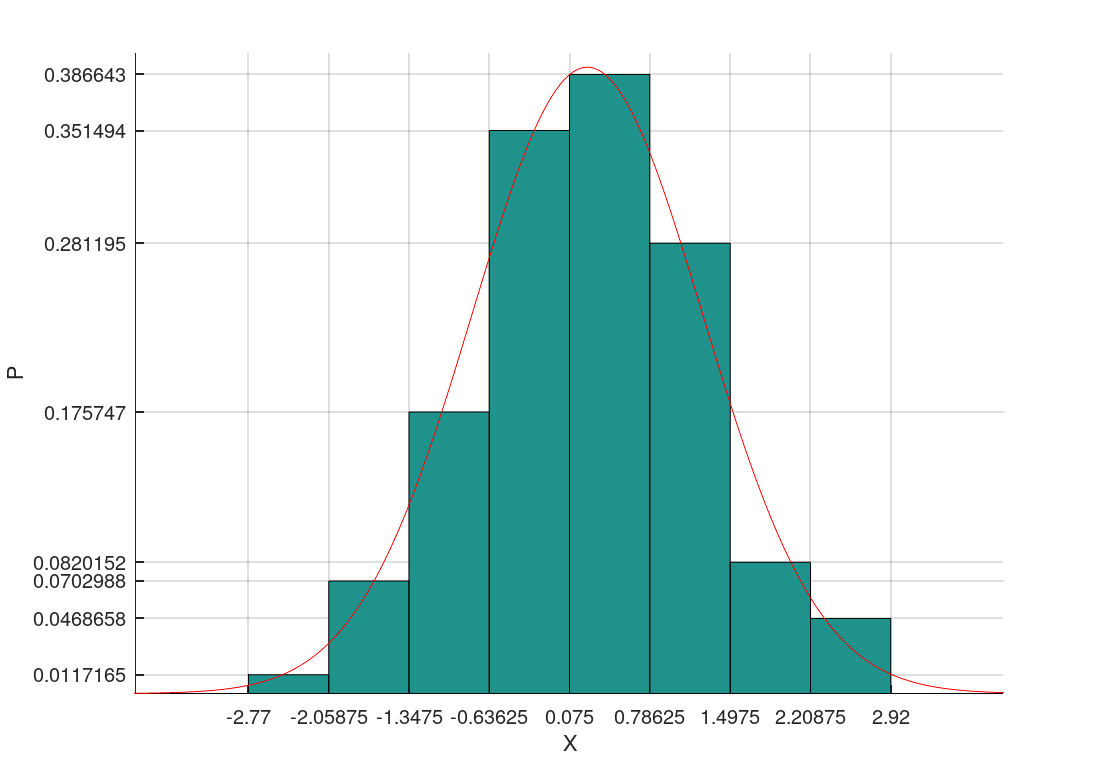
\includegraphics[scale=0.6]{./inc/img/f1.png}
			\caption{Гистограмма и график функции плотности распределения вероятностей нормальной случайной величины с выборочными мат. ожиданием и дисперсией}
	\end{center}
	\label{img:eval}
\end{figure}


\begin{figure}[H]
	\begin{center}

		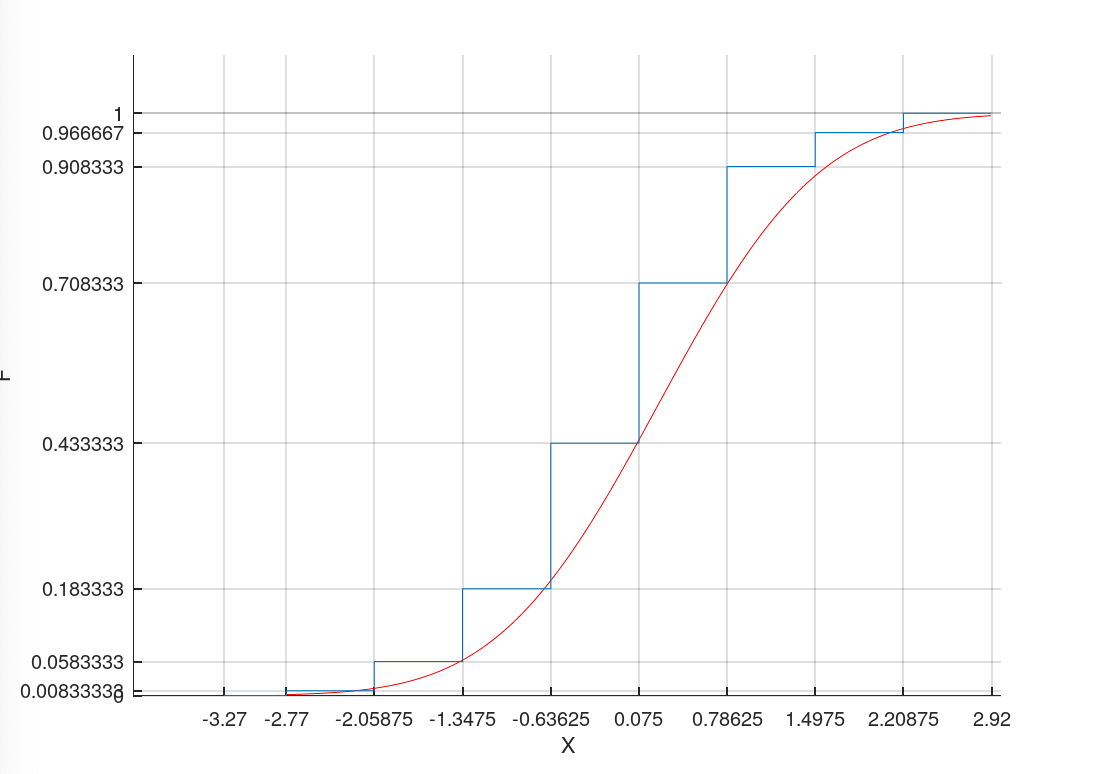
\includegraphics[scale=0.6]{./inc/img/f2.png}
			\caption{График эмперической функции распределения и функции распределения нормальной случайной величины с выборочными мат. ожиданием и дисперсией}
	\end{center}
	\label{img:eval}
\end{figure}


\end{document}